	
\documentclass[varwidth, border=15pt]{standalone}
\usepackage{subcaption}
\usepackage{graphicx}

\usepackage{tabularx} % Addition
\usepackage{multirow} % Addition
\usepackage{booktabs} % Addition
\usepackage[export]{adjustbox} % Addition


% Customize table rendering
\setlength{\tabcolsep}{5pt}
\renewcommand{\arraystretch}{1.3}


\begin{document}
\begin{figure}[t]
\subfloat{
\centering
\adjustbox{valign=t}{
%\hspace{3cm}
\begin{tabular}{llrrrrrrrr}
\toprule
       & Training examples &  49   &  99   &  199  &  398  &  796  &  1593 &  3186 &  6373 \\
       & \% & 0.8   & 1.6   & 3.1   & 6.2   & 12.5  & 25.0  & 50.0  & 100.0 \\
\midrule\bottomrule
\multirow{3}{*}{\rotatebox{90}{F1 score}} & CmBERT &  89.5 &  90.5 &  92.7 &  93.3 &  \textbf{94.1} &  \textbf{94.9} &  \textbf{94.6} &  \textbf{95.1} \\
       & CmBERT-ptrn &  \textbf{92.2} &  \textbf{92.9} &  \textbf{93.6} &  \textbf{93.8} &  93.8 &  94.1 &  \textbf{94.6} &  94.4 \\
       & SpaCy NER &  87.0 &  89.0 &  90.3 &  91.9 &  92.1 &  92.8 &  93.2 &  93.5 \\
\bottomrule
\end{tabular}}
}
\newline
\subfloat{
\centering
\adjustbox{valign=b}{
\centering
         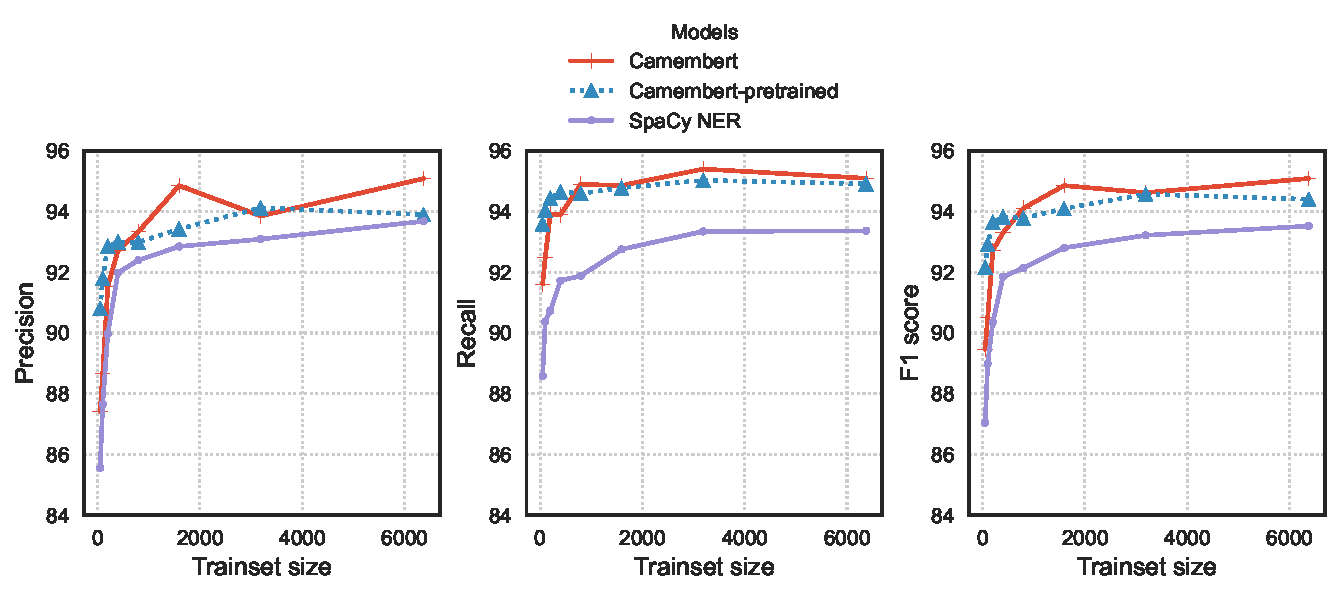
\includegraphics[width=1\textwidth,valign=t]{../images/experiment-1-models-performances.pdf}
         }
}
\end{figure}
\end{document}